%%%%%%%%%%%%%%%%%%%%%%%%%%%%%%%%%%%%%%%%%%%%%%%%%%%%%%%%%%%%%%%%%%%%%%%%%%%%%%%%%%%%%%%%%%%%%%
\begin{toepassing}
	\label{schuifspanning}
Bij een stroming rond een balk met lengte 200mm, breedte 50mm en hoogte 50mm die in de lange richting in de stroming is geplaatst word de druk op de vlakken in de stromingsrichting gemeten. De overdruk aan de voorzijde is uniform 60Pa, aan de achterzijde is dit -20Pa. De stroming oefent een weerstandskracht van 0.5N uit op de balk.

Bepaal de oppervlakte weerstandskracht en de gemiddelde schuifspanning op de zijvlakken van de balk.

	\centering
	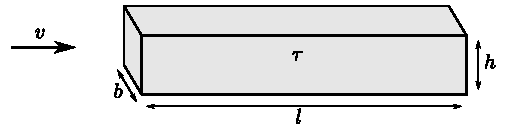
\includegraphics[width=0.48\textwidth]{fig/uitwendige_stroming/schuifspanning.pdf}
\end{toepassing}
\begin{antwoord}{\ref{schuifspanning}}
	$F_s = 0.3N$, $\tau = 7.5N/m^2$
\end{antwoord}
%%%%%%%%%%%%%%%%%%%%%%%%%%%%%%%%%%%%%%%%%%%%%%%%%%%%%%%%%%%%%%%%%%%%%%%%%%%%%%%%%%%%%%%%%%%%%%
\begin{toepassing}[*]
	\label{wolkenkrabber}
Een wolkenkrabber kan vereenvoudigd worden als een balk met grondvlakzijden van 50m en een hoogte van 300m. De weerstandscoëfficiënt van een vierkante sectie is 2.2. Volgens metingen is de gemiddelde windsnelheid afhankelijk van de hoogte volgens $v = C z^{0.40}$. De dichtheid van lucht is 1.22\unit{kg/m^3}.

Indien 3 dimensionale effecten aan de top van de wolkenkrabber verwaarloosd kunnen worden, bepaal dan de totale kracht en het krachtverdeling functie van de hoogte die de wind uitoefent indien op een hoogte van 10m de windsnelheid 5m/s bedraagt.
\end{toepassing}
\begin{antwoord}{\ref{wolkenkrabber}}
	$f = 638 z^{0.8} \unit{N/m}$, $F = 10196\unit{kN}$
\end{antwoord}
%%%%%%%%%%%%%%%%%%%%%%%%%%%%%%%%%%%%%%%%%%%%%%%%%%%%%%%%%%%%%%%%%%%%%%%%%%%%%%%%%%%%%%%%%%%%%%
\begin{toepassing}
	\label{cabrio}
Een cabrio met open dak heeft een weerstandscoëfficiënt van 0.45. Met het dak gesloten is de weerstandscoefficient 0.35.
Bepaal de snelheid waarbij het vermogen nodig om de luchtweerstand te overwinnen met het dak open gelijk is aan het vermogen wanneer de auto met het dak dicht rijdt tegen 100\unit{km/h}. Veronderstel dat het frontaal oppervlak van de cabrio met open en gesloten dak gelijk is.
\end{toepassing}
\begin{antwoord}{\ref{cabrio}}
	$v=92\unit{km/h}$
\end{antwoord}
%%%%%%%%%%%%%%%%%%%%%%%%%%%%%%%%%%%%%%%%%%%%%%%%%%%%%%%%%%%%%%%%%%%%%%%%%%%%%%%%%%%%%%%%%%%%%%
\begin{toepassing}[*]
	\label{airbus}
Een volgeladen Airbus A380 heeft een massa van 650ton, het totale vleugeloppervlak is 845\unit{m^2}. De vleugels zijn opgebouwd uit NACA SC(2) 0610 profielen met een lift en weerstands karakteristiek zoals hieronder weergegeven. De romp vereenvoudigen we als een cilinder met 8m diameter en een weerstandscoëfficiënt van 1.2. De weerstand van de staart en de ophanging van de motoren worden verwaarloosd. De gewenste kruissnelheid is 900km/u. De dichtheid van lucht op de kruishoogte is ongeveer 0.35\unit{kg/m^3}.
		
Bepaal de aanvalshoek van de vleugels nodig voor horizontale vlucht aan kruissnelheid en de stuwkracht die de motoren moeten leveren in deze omstandigheden.

	\centering
	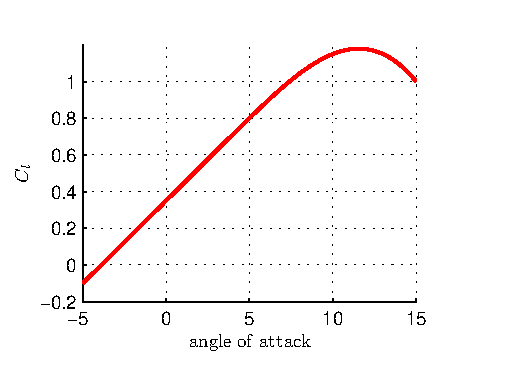
\includegraphics[width=0.48\textwidth]{fig/uitwendige_stroming/NACA_SC(2)_0610_Cl.pdf}
	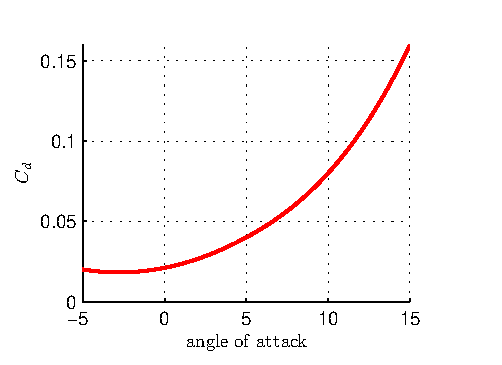
\includegraphics[width=0.48\textwidth]{fig/uitwendige_stroming/NACA_SC(2)_0610_Cd.pdf}
\end{toepassing}
\begin{antwoord}{\ref{airbus}}
	$\alpha \approx 4\deg$, $F \approx 983\unit{kN}$
\end{antwoord}
%%%%%%%%%%%%%%%%%%%%%%%%%%%%%%%%%%%%%%%%%%%%%%%%%%%%%%%%%%%%%%%%%%%%%%%%%%%%%%%%%%%%%%%%%%%%%%


\section*{Antwoorden}
	\begin{multicols}{2}
		\includecollection{antwoorden}
	\end{multicols}